\chapter{Backend}
\label{chap:Backend}

\textbf{Aidan: I might have 'abused' of the word-connected-to-another form. Because it made sense to me. Please let me know what do you think.}

In this chapter we describe the details of our system per \autoref{fig:architecture}.
As was mentioned before, our implementation works as a backend that sits between the user interface and a remote SPARQL query endpoint.

Since we are focusing on dealing with large datasets (480GB for the uncompressed Wikidata dump), direct in-memory storage/query is not possible, and a specialized index is required. Our index differs from a SPARQL Endpoint index in that for each triple's \textit{Property}, our index does not store the values of the \textit{Entities} linked to that \textit{Property}, but rather the \textit{Types} of those \textit{Entities}. This removes the one-to-one relation in triples, thus creating approximation of the possible available values while improving query times.

Our system will work in two phases: First our specialized index must be built and second, queries will be processed. We will first present a system overview and afterwards an example.

As an overview for our index, given a dataset with triples in the form: 

\begin{minted}[linenos,tabsize=2,frame=single,samepage]{sparql}
<entity1> <type> <type1> . 
<entity1> <type> <type2> .
<entity1> <property1> <entity2> .
<entity1> <property2> <entity3> .
[...]
<entity2> <type> <type3> .
[...]
<entity3> <type> <type4> .
[...]
\end{minted}

Our system will build two indexes. First an \textit{entities} index with the following structure:
\begin{minted}[linenos,tabsize=2,frame=single,samepage]{text}
entity1.Type = [type1,type2,...]
entity1.Properties = [property1, property2,..]
[...]
entity2.InverseProperties = [property1,..]
[...]
entity3.InverseProperties = [property2,..]
\end{minted}

And then a \textit{properties} index with the following structure:
\begin{minted}[linenos,tabsize=2,frame=single,samepage]{text}
property1.Domain = [type1,type2,...]
property1.Range = [type3,..]
[...]
property2.Domain = [type1,type2,...]
property2.Range = [type4,..]
\end{minted}

Once the index is built, queries can be processed. When given a query graph, our system will first check all the graph's nodes and edges for constants\footnote{We will further on see what a constant is.}. For each constant element, we will annotate that element: Nodes with the types of that constant; Edges with the constant's domain- and range-types. 

\textbf{Aidan: Domain and range were introduced in the first chapter, should I repeat again it here?}

At this stage, we have information about the types of some nodes and edges. This gives our system some data about variable-nodes and -edges linked to known constants. This means that at this point, we can provide approximated suggestions for every element that links to our known constants. The next step is to intersect the inferred types and finally, provide relevant instances of those inferred types. 

Intersecting types is required to match the information we know about linked constants. If a node, for instance, has incoming and outgoing edges, the possible types of that node will be the ones that are a possible match for all of those edges. Since we may know the domain- and range-types of some of the edges, we can estimate that the possible types for a node, would be those in the intersection of the incoming-edges-range-types and the outgoing-edges-domain-types.

\textbf{Aidan: Should I remove the detail of the previous paragraph? Or rephrase/remove the 'interesect' in the paragraph before this one? The idea might be already clear before, but "intersecting" is mentioned.}

We have prepared an example to guide our readers on the query processing. Let us jump into it.

With this example at hand, we will now proceed to explain the bits and pieces of our backend. The system is composed of four modules, here ordered by their relevance to the system: 
The entities and properties index,
a query parser module,
a graph exploration module and
a query execution module. 
An additional application interface (API) acts as the entry point for our system.

This chapter starts off by detailing the specialized index.
The index section includes the pre-processing and indexing of an RDF dataset dump.

We will then proceed by describing the graph parser module, which converts an input to our own data structure. 
In our case, a graph data structure is used to store our SPARQL statements. 
In this graph, the nodes will represent statements' \textit{subjects} and \textit{objects}, while edges represent \textit{predicates}. 

This graph is then processed by the graph exploration module. 
At this stage, basic information about the nodes, edges and certain relations between them are identified and added to the data structure. 
With this information in place, the graph is passed on to the query execution module. 

The execution of the query is sent in parallel to both the remote SPARQL endpoint and the local index. 
The request to the remote end is sent with a configurable timeout, usually of a few seconds. 
If the remote SPARQL endpoint returns values within this time, these results will be returned; otherwise, the specialized local index results will be post-processed and returned. 

The local index will return information about certain \textit{entity types}, \textit{instances} and \textit{properties}. 
These results will be processed; mainly some intersections and duplication removal is required at this stage.
The post-processed results are then sent back to the user for display and selection.

This double request mechanism allows us to deliver exact results in the case the remote SPARQL endpoint does not time out, or otherwise, the over-approximated results from our local index in case it does time out. 
Thus the system can return possible results that would otherwise keep the user indefinitely waiting or in the worst case, never return. 

The chapter concludes by describing our application interface, which works as the entry point of our system. 
It will take requests from different services, such as SPARQL query editors or SPARQL visual explorers and send the information either to the graph parsing module, for SPARQL queries; 
or directly to the index, for keyword search. 
The integration with a user interface will be left for \autoref{chap:Frontend}.

% ##############################################################################################
% ##############################################################################################
% ##############################################################################################

\section{Initializaton}
\label{chap:init}

Before indexing the data, some pre-processing is required. 
The pre-processing filters what are considered valid triples and adds certain inverse relations between some of the triples that are read. 
The system will process a RDF dump to do the following changes to it:
\begin{itemize}
    \item Filter valid triples.
    \item Add inverse relations.
    \item Sort the file.
\end{itemize}

\begin{figure}[H]
    \centering
        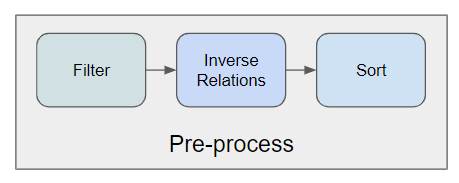
\includegraphics[width=0.5\linewidth]{imagenes/Preprocess.png}
        \caption{Pre-processing workflow}
        \label{fig:preprocess}
\end{figure}

Another important aspect of the system, is that it takes compressed files as inputs, and generates compressed output files. 
This is important mainly due to space restrictions. 
The Wikidata dump\footnote{As per February 2020} is $\sim$36GB compressed and $\sim$480GB decompressed.
A pre-processed output file is $\sim$8GB compressed. 

\subsection{Filter}

The first pre-processing task is to filter the input data. 
We will focus on Wikidata labels and descriptions in the English language. 
We will also remove triples with datatype values or external IDs.
While this step could be optional, it helps to reduce the number of triples that the system will have to index later. 
Multiple filtering criteria are implemented in the system. 
At the current development stage, these criteria are hard-coded, but they could be extended to use regular expressions or other types of filtering rules. We have left this as a point of future work.

We include triples that match the following rules in our data:
\begin{itemize}
    \item Where \textit{subject} starts with \texttt{http://www.wikidata.org/entity/}.
    \item Where \textit{predicate} starts with \texttt{http://www.wikidata.org/prop/direct/} 
            \subsubitem and \textit{object} starts with \texttt{http://www.wikidata.org/entity/}.
        \subitem or \textit{predicate} is \texttt{label}, \texttt{description} or \texttt{alt-label} 
            \subsubitem and \textit{object} is \textit{literal} and ends with \texttt{@en}.
\end{itemize}

\begin{example}
We now present some examples of both filtered and non-filtered triples.
We have used prefixes when required for shortening lines.

Filtered triples:
\begin{minted}{SPARQL}
#Entity or Property Subject, Label predicate in english:
wd:Q27 rdfs:label "Ireland"@en .
#Entity or Property Subject, Description predicate in english:
wd:Q147 schema:description "young of a cat"@en .
#Entity or Property Subject, Alternative Label predicate in english:
wd:P22 skos:altLabel "dad"@en .
#Entity subject, Property predicate, Entity subject triples:
wd:Q465 wdt:P277 wd:Q251 .
\end{minted}

Non-filtered triples:
\begin{minted}{SPARQL}
#Non-english literal objects:
wd:Q27 rdfs:label "Irlanda"@it .
#Non -Label, -Description or -AltLabel predicates:
wd:Q298 skos:prefLabel "Chile"@en .
wd:Q348 <http://www.wikidata.org/prop/direct-normalized/P349> <object> .
#Non-Entities or -Property subjects:
<http://wikiba.se/beta#Dump> <http://schema.org/softwareVersion> "0.1.0" .
<https://www.wikidata.org/wiki/Special:Entity/Q27> rdfs:label "Irland"@en .
#Non-literal or -entity objects:
wd:Q47 wdt:P1082 "1852168"^^<http://www.w3.org/2001/XMLSchema#decimal>
\end{minted}
\end{example}

\subsection{Inverse relations and sorting}

Following the filtering process, the system adds the inverse relation for triples patterns containing non-literal objects. 
For every \texttt{(subject, predicate, object)} triple with only non-literal \texttt{objects}, the system adds the inverse \texttt{(object, inverse/Predicate, subject)} triple. This will allow us to treat the subject and object positions of triples equally for the purposes of generating suggestions, while requiring minimal additional code in later components.

\begin{example}
For example, the following triples:

\begin{minted}{SPARQL}
<uri:/subjectA> <uri:/type> <uri:/subjectTypeB> .
<uri:/subjectA> <uri:/predicate> <uri:/objectC> .
\end{minted}

Produces a new file with the original triples, plus the new inverse relation triples:

\begin{minted}{SPARQL}
<uri:/subjectA> <uri:/type> <uri:/subjectTypeB> .
<uri:/subjectA> <uri:/predicate> <uri:/objectC> .
[...]
<uri:/subjectTypeB> <uri:/inverse/type> <uri:/subjectA> .
[...]
<uri:/objectC> <uri:/inverse/predicate> <uri:/subjectA> .
\end{minted}

The separation $[...]$ between \textit{subject}, \textit{object} and \textit{subjectType} statements are due to the final pre-processing task: sorting the output dump file. 
This keeps entity related triples grouped together, which in turn makes indexing more efficient.

\end{example}

The second benefit of this approach, is that with this sorting, finding if an \textit{entity} is a \textit{type} is immediate, since it will contain predicates as \textit{/inverse/type} within its triples. 
The pre-processing could exclude this step; nevertheless, adding the inverse triples significantly reduces indexing time, while without it, several iterations through disk access would have been required. 

The final step is to sort the pre-processed file. Sorting is done via merge sort. At the current development stage, the process is called from the command line. It is to be noted that for sorting of the file, $\sim$3$\times$ the size of the input file is required as free disk space. The command used for sorting is as follows: 

\begin{verbatim}
    gzip -dc {input} | LANG=C sort                      \
         -S 200M                                        \
         --parallel=4                                   \
         -T tmp/                                        \
         --compress-program=gzip | gzip > {output}
\end{verbatim}

This command takes an \texttt{\{input\}} compressed file as parameter. It sorts it using the \texttt{tmp/} folder for storing temporary files, where each chunk during the merge-sort process is as large as 200 Mbytes. During the process, it uses 4 threads. Finally the sorted results is compressed to an \texttt{\{output\}} file.

% ##############################################################################################
% ##############################################################################################
% ##############################################################################################

\section{Index}

After a pre-processed dump has been created, the system can start indexing it. 
Indexing occurs in two steps: once for entities and once for properties. In the end, two indexes are created, one for each.

Entity indexing involves the following steps:
\begin{itemize}
    \item Rank entities via PageRank
    \item Index entities
\end{itemize}

Properties indexing has the following steps:
\begin{itemize}
    \item Rank properties by frequency
    \item Build a domain dictionary
    \item Build a range dictionary
    \item Index properties
\end{itemize}

A depiction of both of these processes can be seen in \autoref{fig:indexing}.

\begin{figure}[H]
    \centering
        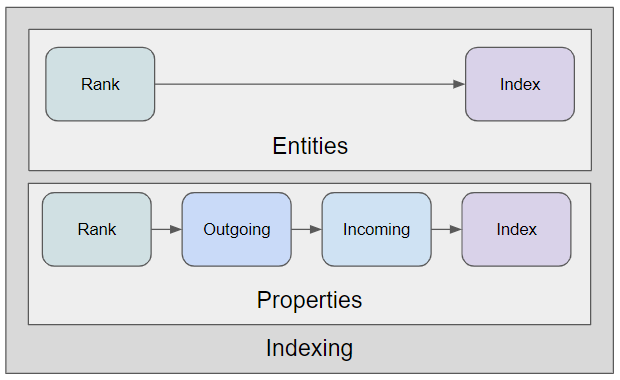
\includegraphics[width=0.7\linewidth]{imagenes/Indexing.png}
        \caption{Indexing workflow}
        \label{fig:indexing}
\end{figure}

\subsection{Entities}

\subsubsection{Inverted Index}

After calculating the ranking values for the graph-modelled input data, the data is indexed using \textit{Lucene}. 
As seen in \autoref{chap:lucene}, Lucene is a search engine library, mostly suitable for text indexing and searching capabilities. 
This enables out-of-the-box keyword-search for entities and properties.
As mentioned previously, Lucene adds an additional relevance metric based on TF-IDF, which complements our previously calculated PageRank value.

The index in Lucene is a document database index. 
Each document of this database has fields. 
In our case, each document corresponds to an \textit{Entity} and each \textit{Entity} has fields such as \textit{Label}, \textit{Description} or a collection of \textit{Properties}. 
We now present each \textit{Field} that every Document in our index has, and the description of those \textit{Fields}.

Each entity-document contains the following fields:
\begin{itemize}
    \item \textbf{Id:} String field. The IRI of the entity. In our case, it is stored without the prefix. For Wikidata, this identifier is a letter \texttt{Q} followed by the identification number.
    \item \textbf{Label:} Text field.  Value that represents a name for the resource (that may be ambiguous).  In the dump, the label is the value of the triples with the predicate \url{http://www.w3.org/2000/01/rdf-schema#label}. 
    \item \textbf{AltLabel:} Text field. Other names the resource is known by.  The predicate for these values in the dump is \url{http://www.w3.org/2004/02/skos/core#altLabel}. This field can store multiple values for the same document.
    \item \textbf{Description:} Text field. Small description of the resource, which helps to disambiguate the resource from others with the same or similar labels. Triples with a description have the predicate \url{http://schema.org/description}.
    \item \textbf{InstanceOf:} String field. Indicates if the entity is a type. For example, \textit{Barack Obama (Q76)} is type \textit{Human (Q5)}. \textit{Human} has a \textit{InstanceOf} field with a \textit{"true"} value. This is based on having a predicate \texttt{inverse/instanceOf (P31)}. This is possible due to adding the previously mentioned inverse relation for predicates in the pre-processing stage.
    \item \textbf{Property:} String field. The collection of the outgoing properties that this resource has. This field can store multiple values. All values in this field are stored without their prefix. Property predicates start with  \url{http://www.wikidata.org/prop/direct/}
    \item \textbf{InverseProperty:} String field. Same as the Property field, but for incoming properties. As was mentioned before, these triples were added in the pre-processing step to the dump file.
\end{itemize}

\subsubsection{Ranking}

Lucene offers relevance-based ranking (using a variant of TF-IDF) for searches. But we need importance too: A user might be searching for the term 'Obama'. The reader might think about \textit{Barack Obama} as a first suggestion, but \textit{Tom Obama} or \textit{Mount Obama} might have the same relevance in terms of TF-IDF and keywords, but on is much more important than the other.

In order to get the results sorted by both relevance and importance, a ranking value, calculated via PageRank, is added to our index. 
As seen in \autoref{chap:pagerank}, PageRank was originally designed for directed graphs such as websites and their links. 
PageRanks works by iteratively setting relevance values on nodes based on the incoming and outgoing nodes (edges pointing to other nodes). 
In the same way, our PageRank implementation works by iteratively setting the relevance of incoming and outgoing entities through their properties. 

Our implementation of PageRank works in memory, and is not different from other implementations. 
Due to the amount of data, for our implementation we have considered using value types (e.g.: \texttt{int, double, arrays}) instead of more complex reference types (e.g.: \texttt{List, Dictionary, etc.}) in favor of performance. 
Twenty iterations have been considered for this ranking process.

PageRank values are store in the index as \textit{Lucene's Boost}. This helps Lucene to sort the results of a query by their importance, as well as relevance. PageRank values are stored in both the \textit{Label} and \textit{AltLabel} fields.

\begin{example}
As an example, a collection of triples from a single entity is presented. Its indexed document and field representation is also presented. We have taken a partial sample of the Universe (Q1) as an example reference.

\begin{minted}{SPARQL}
wd:Q1 schema:description "totality of space [...]"@en .
wd:Q1 rdfs:label "Universe"@en .
wd:Q1 skos:altLabel "Our Universe"@en .
wd:Q1 skos:altLabel "The Cosmos"@en .
wd:Q1 wdt:P31 wd:Q36906466 .
wd:Q1 wdt:P361 wd:Q3327819 .
wd:Q1 wdt:P793 wd:Q323 .
wd:Q1 wdt:P828 wd:Q323 .
wd:Q1 <http://www.wikidata.org/prop/reverse/P1542> wd:Q323 .
\end{minted}

The index document representation for this triples is in \autoref{table:triplesToDocument}.

\begin{table}[h!]
\centering
\begin{tabular}{ll}
Field           & Value                    \\ 
\hline
Id              & Q1                       \\
Label           & Universe                 \\
AltLabel        & Our Universe             \\
AltLabel        & The Cosmos               \\
Description     & totality of space [...]  \\
InstanceOf      & Q36906466                \\
Property        & P361                     \\
Property        & P793                     \\
Property        & P828                     \\
InverseProperty & P1542                   
\end{tabular}
\caption{Document and field representation of example triples}
\label{table:triplesToDocument}

\end{table}

\end{example}

\subsection{Properties}
The next step in the initialization stage is to create an index for the properties contained in the input dataset.

\subsubsection{Inverted Index}
As  was done with the \textit{Entities Index}, an \textit{Index} for the input \textit{Properties} is also created. In this case, each document corresponds to a \textit{Property} and each \textit{Property} has fields such as \textit{Label}, \textit{Description} or a collection of \textit{Domain} and \textit{Ranges}. 
We now present each \textit{Field} in our index, and the properties of those \textit{Fields}.

Each property-document contains the following fields:
\begin{itemize}
    \item \textbf{Id:} String field. The IRI of the property. In our case, it is  stored without the prefix. For Wikidata, this identifier is a letter \texttt{P} followed by the identification number.
    \item \textbf{Label:} Text field.  Value that represents a name for the resource.  For the properties in the dump, the same predicate (\url{http://www.w3.org/2000/01/rdf-schema#label}) is used for labels. 
    \item \textbf{AltLabel:} Text field. Other names the resource is known by. The predicate for these values in the dump is \url{http://www.w3.org/2004/02/skos/core#altLabel}. As in the entities index, this field can store multiple values for the same document. Frequency relevance values are stored here as well. This helps Lucene to sort the results of a query by their relevance.
    \item \textbf{Description:} Text field. Small description of the resource, which helps users to disambiguate the resource from others with the same labels. Triples with a description have the predicate \url{http://schema.org/description}.
    \item \textbf{Domain:} String field. The collection of the entity-types that direct \textit{from} this resource. This field can store multiple values. All values in this field are stored without their prefix.
    \item \textbf{Range:} String field. The collection of the entity-types that direct \textit{to} this resource. This field can store multiple values. All values in this field are stored without their prefix.
\end{itemize}

\subsubsection{Ranking}
For ranking \textit{Properties}, the frequency of appearance is used as our relevance metric. 
We are using frequency since PageRank, which is good for ranking nodes in a directed graph, is not very good for ranking edge labels.
In order to calculate these values, a \textit{Dictionary} is built with the \textit{Key} being the \textit{PropertyId} and the \textit{Value} being the amount of times this property appears in the dataset.

Frequency relevance values are used as \textit{Lucene's Boost}. This helps Lucene to sort the results of a query by relevance. The Boost values are added again to both \textit{Label} and \textit{AltLabel} fields.

\subsubsection{Type Domains}

Given a triple pattern statement, \textit{Type Domains} allow the system to provide suggestions in the follow two scenarios:
\begin{itemize}
    \item Given a \textit{Property}: The system provides suggestions for the \textit{Subject}.
    \item Given a \textit{Subject}: The system provides suggestions for the \textit{Property}.
\end{itemize}

\textit{Type Domains} work by creating a \textit{Dictionary} with \textit{PropertyId} as \textit{Key} and all the \textit{TypeIds} that each \textit{Property} has as \textit{Domain}.

\begin{example}
Given the following data:
\begin{minted}{SPARQL}
<uri:/BarackObama> <uri:/instanceOf> <uri:/Human> .
<uri:/BarackObama> <uri:/bornIn> <uri:/Honolulu> .
\end{minted}

And given the following triple pattern:
\begin{minted}{SPARQL}
?var1 <uri:/bornIn> ?var2 .
\end{minted}

As suggestions for \texttt{?var1} the system provides instances of \texttt{Human} as suggestions, sorted by relevance. Among the results \texttt{BarackObama} can be found.

This type of query usually times out when run on the remote endpoint (when no or not low enough \texttt{LIMIT} statement is present) and will not offer ranked options. This feature of our system will provide users ranked suggestions in a predictable amount of time.
\end{example}

\begin{example}
Given the following data:
\begin{minted}{SPARQL}
<uri:/BarackObama> <uri:/instanceOf> <uri:/Human> .
<uri:/BarackObama> <uri:/bornIn> <uri:/Honolulu> .
\end{minted}

And given the following triple pattern:
\begin{minted}{SPARQL}
<uri:/BarackObama> ?prop1 ?var2 .
\end{minted}

As suggestions for \texttt{?prop1} the system provides properties that direct outwards from instances of \texttt{Human}, sorted by frequency. Among the results \texttt{bornIn} can be found.

It is worth mentioning that for this scenario, the baseline system queries the remote endpoint, which returns the properties only available for \texttt{BarackObama}. In case that this query fails, our system would do as mentioned before and return the results from our local index.
\end{example}

\subsubsection{Type Ranges}

Given a triple pattern statement, type ranges allow our system to provide suggestions in the following two scenarios:
\begin{itemize}
    \item Given a \textit{Property}: The system provides suggestions for the \textit{Object}.
    \item Given an \textit{Object}: The system provides suggestions for the \textit{Property}.
\end{itemize}

\textit{Type Ranges} work in a similar way as \textit{Type Domains}: By creating a \textit{Dictionary} with \textit{PropertyId} as \textit{Key} and all the \textit{TypeIds} that each \textit{Property} has as \textit{Range}.

\begin{example}
Given the following data:
\begin{minted}{SPARQL}
<uri:/BarackObama> <uri:/bornIn> <uri:/Honolulu> .
[...]
<uri:/Honolulu> <uri:/instanceOf> <uri:/City> .
\end{minted}

And given the following triple pattern:
\begin{minted}{SPARQL}
?var1 <uri:/bornIn> ?var2 .
\end{minted}

As suggestions for \texttt{?var2} the system provides instances of \texttt{City} as suggestions, sorted by relevance. Among the results \texttt{Honolulu} can be found.

This type of query times out on a SPARQL endpoint in most cases. As in the \textit{Type Domain} example, this indexed feature will once again will provide users ranked suggestions in a predictable amount of time.
\end{example}

\begin{example}
Given the following data:
\begin{minted}{SPARQL}
<uri:/BarackObama> <uri:/bornIn> <uri:/Honolulu> .
[...]
<uri:/Honolulu> <uri:/instanceOf> <uri:/City> .
\end{minted}

And given the following triple pattern:
\begin{minted}{SPARQL}
?var1 ?prop1 <uri:/Honolulu> .
\end{minted}

As suggestions for \texttt{?prop1} the system provides properties that direct to instances of \texttt{City}, sorted by frequency. Among the results \texttt{bornIn} can be found.

In contrast to what was described for the type domains, these values are not always returned before timeout from the remote endpoint. This feature of our system will provide users ranked suggestions in a predictable amount of time.
\end{example}

\section{Query Parser}
\label{chap:parser}

Once both entities and properties have been indexed, the system can go into online mode. After receiving a user request, the first action of the system is to parse the given request.

We have previously mentioned that the system can work in two ways: keyword search and query term suggestions. Keyword search is quite straightforward: A keyword is given and the inverted index searches and returns the relevant values. These requests go directly to the inverted index, which in turn returns the desired results. No further processing is involved.

Regarding the query term suggestions, there are two possible inputs that the system can take:
\begin{itemize}
    \item \textbf{Query as a graph:} A graph object is passed to our system. This integrates better with graphical user interfaces, such as RDFExplorer.
    \item \textbf{Query as text:} A SPARQL query is passed to our system. This approach is most suitable for text query clients, such as the Wikidata Query Endpoint.
\end{itemize}

For both query term suggestion cases, the goal of the \textit{Query Parser} is to convert the input into a graph data model.

In SPARQL query input scenarios, the input query text is converted using the following triple pattern rules:
\begin{itemize}
    \item Only \texttt{SELECT WHERE} queries are supported in the current version. The system will ignore the \texttt{SELECT} variables and take the \texttt{WHERE} statements.
    \item Each triple pattern statement follows a \texttt{Subject Predicate Object} construction.
    \item Each term can be either a constant or a variable.
    \item Each variable will start with the question mark character \texttt{?}. E.g.: \texttt{?var1, ?prop7}
    \item Each constant can be either an IRI in the form of \texttt{<http://iri>} or \texttt{prefix:iri}, when the prefix is given.
\end{itemize}

Given such inputs, parsing an incoming request is straightforward and the queries are converted to the input graph.

% ##############################################################################################
% ##############################################################################################
% ##############################################################################################

\section{Graph Exploration}
\label{chap:graph_exploration}

After a request has been received and the data has been converted into the graph data model, the system explores this graph to check existing relations between nodes and edges. 

The first step of the graph exploration process checks the following:
\begin{itemize}
    \item Which nodes and edges are variables and which are constants.
    \item Which variable nodes have an \texttt{instanceOf} outgoing edge.
\end{itemize}

As a first step, all edges are marked as constant or variable: 
If an edge has a given URI, then that edge is considered a constant, otherwise a variable. 
All nodes are checked in the same manner: If a node has a provided URI, then that node is considered to be a constant, otherwise it is considered to be a variable. 

The next step is to mark the variable nodes as \texttt{instanceOf}:
If a node is the source of an \texttt{instanceOf} property edge, then the node is considered as an \texttt{instanceOf}. To expand on this, let us consider the following statement: \texttt{?var1 instanceOf Human}. As a remark for this case, no other incoming and outgoing edges are available for \texttt{?var1}.

We can summarize this graph exploration with the following code:
\begin{minted}[linenos,tabsize=2,frame=single,samepage]{csharp}
ExploreGraph (graph) {
  //We will start by the edges:
  foreach (edge in graph.Edges) {
    //If the edge has a given URI, then it is a constant:
    if (edge.HasURIs())
      edge.IsConstant = true;
    //If the URI is instanceOf, then we mark it as such:
    if (edge.HasInstanceOfURIs())
      edge.IsInstanceOf = true;
  }
  //Then with nodes, same as before:
  foreach (node in graph.Nodes) {
    if (node.HasURIs())
      node.IsConstant = true;
    //Now we check the outgoing edges.
    //If any outgoing edges is InstanceOf, then the node is also:
    foreach (outEdge in node.OutgoingEdges)
      if (outEdge.IsInstanceOf)
        node.IsInstanceOf = true;
  }
}
\end{minted}

As last step we check if the input query has enough valid information. We first check if the input is conformed by multiple disconnected sub-graphs. If so, we evaluate each disconnected sub-graph to find if any constant are given in that sub-graph. Consider the following example: \texttt{?v1 ?p1 ?v2 . ?v2 ?p2 ?p3 .}. 
In the two statements, only variables and no constants are provided.
Since a plethora of values could be returned for this sub-query, our system avoids this sub-graph and lets the remote SPARQL endpoint decide which values should be returned in such cases.

The graph exploration allows us to annotate certain nodes and edges, and consider them valid for query execution. To summarize the different exploration scenarios:
\begin{itemize}
    \item Nodes and edges are classified as constants or variables: If a node or edge is a constant, then do not return any values for it.
    \item Nodes and edges are classified as \texttt{instanceOf}.
    \item \texttt{instanceOf} nodes with no incoming or outgoing edges, are directly queried on our local index.
    \item Sub-graphs with only variables, no constants are directly queried on the SPARQL endpoint.
\end{itemize}

Once all nodes and edges have been annotated, our system will proceed to evaluate the graph query and fetch the suggestions. 

% ##############################################################################################
% ##############################################################################################
% ##############################################################################################

\section{Query Execution}
\label{chap:execution}

The goal of our Query Execution module is to get results for our graph's nodes and edges: User's entities and properties. The results will be retrieved from either the local index or the remote endpoint, but a request will be sent to both, with priority on the remote endpoint. In other words, we will query the remote endpoint for exact results: if it times out, the local approximated results will be returned.

Before diving into the details of how the results are retrieved, we will present an example that covers what we have seen so far and what comes ahead.

\begin{example}

Let us consider that a user is looking for "siblings that have directed a film together". 
Since the user might not very familiar with the available properties in a dataset such as Wikidata, it would be hard for them to directly specify the properties they require. Let us consider that they have built a graph such as the one in \autoref{fig:example_graph4}:

\begin{figure}[H]
    \centering
        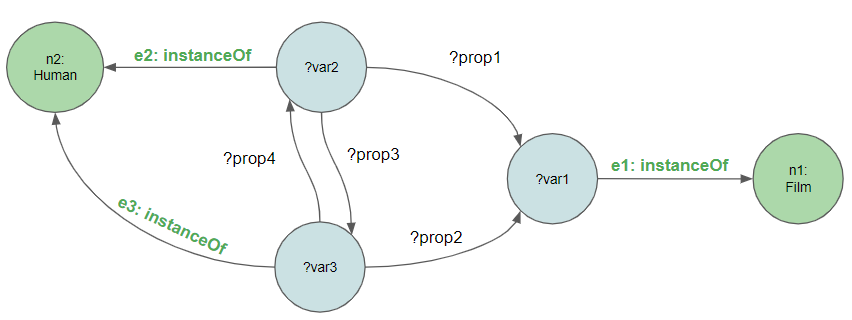
\includegraphics[width=\linewidth]{imagenes/ExampleGraph1.png}
        \caption{Example graph: Siblings that have directed a film together}
        \label{fig:example_graph4}
\end{figure}

Building such a query in a Visual query builder, such as RDFExplorer; or directly into the Wikidata Query Service, will timeout since the graph pattern is quite complex and has many variables that can match millions of nodes in the data. Our goal in such an scenario is to provide users with over-approximated suggestions, so that they can assign values to the variables until the query does not time out and the correct results are provided.

\textbf{Aidan: Should I add the SPARQL query in the exampe above? (Would mean that the user knows about Human or Film but not the properties)}

Let us go through how our system will process this query. 
As a first step, our system will explore the graph to retrieve information about it:
\begin{minted}[linenos,tabsize=2,frame=single,samepage]{text}
n1, n2 are constants (Film, Human);
e1, e2, e3 are constants (instanceOf);
?var1 is an instance of type Film;
?var2, ?var3 are instances of type Human;
\end{minted}

Since we already have enough information about all \texttt{?var1}, \texttt{?var2} and \texttt{?var3}; our proposals for these variables are currently limited to instances of those types: instances of Human and Film. As readers might suspect, there are millions of values that these individual variables can take. 

Our system will support users in narrowing the options for the rest of variables: the properties, which in turn support our users in completing the missing information in the graph.

Looking at the graph, we can make the following observations:
\begin{minted}[linenos,tabsize=2,frame=single,samepage]{text}
?prop1, ?prop2 have domain Human and range Film;
?prop3, ?prop4 have domain and range Human;
\end{minted}

Our index contains the domain- and range-types for all properties, from here we know: for each type, the incoming and outgoing properties. 
We can use this information at this point to annotate that each variable-property must be both in the incoming-properties for the target-node-type and the outgoing-properties for the source-node-type.

Let us ground this last paragraph with some focus on our given example. Let us focus on \texttt{?prop1}. The following is noted by our system:
\begin{minted}[linenos,tabsize=2,frame=single,samepage]{text}
?prop1 has target ?var1 and source ?var2;
?var1 is instance of type Film;
Type Film has a collection of incoming properties: FilmInProps;
?var2 is instance of type Human;
Type Human has a collection of outgoing properties: HumanOutProps;
?prop1 must be in the intersection of FilmInProps and HumanOutProps;
\end{minted}

Using the previous process, we can now provide a list of proposals to our users:
\begin{verbatim}
    ?prop1, ?prop2: [directedBy, actsIn, producedBy, ...]
    ?prop3, ?prop4: [motherOf, fatherOf, sonOf, siblingOf, ...]
\end{verbatim}

At this stage, a user can select from an approximated suggestions list their wished property. 
Every time new information is added to the query graph, the query is sent to the remote SPARQL endpoint, in our case Wikidata. 
Since more properties and entities are now assigned, the query will not time out and the exact results will be provided to the user.

\end{example}

It is to be mentioned that, since we do not know if the remote endpoint will time out, both queries are send in parallel threads. The remote endpoint query is sent right after the graph exploration. The local query requires some graph traversal. In this traversal, relationships between constant nodes and edges are projected over other elements.

In our experience while testing our system, we have acknowledged that some user queries can be sent to the remote SPARQL endpoint and the response can come in a fraction of a second, while others can take minutes or timeout. 
We have run several tests with different values and the response time can vary significantly for the same query at different times. While this is actually hard to measure, probably due to Wikidata caching the user queries, creating parallel threads for both local and remote queries helps get timed results.

\textbf{Aidan: Not sure if include last paragraph (but I will write about it in the conclusions)}

In this section we will go into more detail about how both queries are built and sent. First, the details of the remote endpoint requests are revised, to end with the local index.

\subsection{Remote Endpoint Requests}

As was mentioned before, after processing the user query, it is sent to the remote endpoint. Since the focus is on enriching the user experience, in order to send the queries to the remote endpoint, the query is first simplified.

During our tests we have realized that using services such as the \textit{Wikidata Label Service}, or querying for labels, can dramatically increase the query response time and timeout for several queries. In order to overcome this and provide the users with useful information about the queried entities, the label and description for all the endpoint results are retrieved from the local index.

Additionally each disconnected sub-graph query will be sent independently. This also allows some values to return when some part (or sub-graph) of the query takes too long or fails and also avoids a Cartesian product when running disconnected sub-graphs in the same query.

\textbf{Aidan: Not sure if the cartesian product applies now that disconnected subgraph is mentioned}

Finally, filters and operators that may exist in the query are removed. While we acknowledge that this has a dramatic impact on the intent of the query, we have considered that this could be included in future versions of the system, and it is not included for now.

The following modifications are handled:
\begin{itemize}
    \item A query will be sent for each disconnected sub-graph.
    \item Both labels and descriptions for each element are added from the local index.
    \item Filters and operators are removed from the query.
\end{itemize}

With the previous conditions at hand, the system will send the request to the endpoint and wait for the response.

\subsection{Access to Local Index}

For the local specialized index, additional graph exploration is required. The goal is: if an edge is constant, project the edge's domain- and range-types onto the adjacent variable-nodes; if a node is constant, project the node-types onto the incoming- and outgoing-variable-properties.

At the start of this chapter we presented the example  "siblings that have directed a film together" (\autoref{fig:example_graph4}): We covered the variable suggestions while given some constants and \texttt{instanceOf} edges. We explained how by providing suggestions, users could complete their queries with approximate suggestions until the remote endpoint returned exact results before timeout. 

In this section, we are going to explain in more detail how we do our final graph exploration and which results we will get from our local index. For this, we will go from a simple graph pattern to more complex one.

\begin{example}
Let us consider the graph of \autoref{fig:example_graph1}.

\begin{figure}[H]
    \centering
        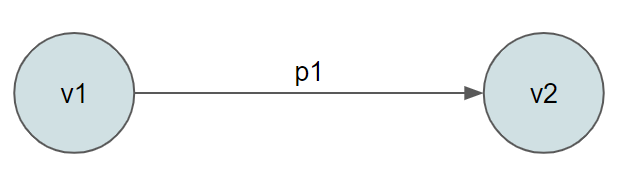
\includegraphics[width=0.5\linewidth]{imagenes/graph1.png}
        \caption{Local index access for a simple graph.}
        \label{fig:example_graph1}
\end{figure}

The graph on \autoref{fig:example_graph1} can be described by the following triple pattern: \texttt{v1 p1 v2}. If all of the elements are variables, we would let the remote endpoint handle this case (as was described in \autoref{chap:graph_exploration}). In other words, we will assume that something in this graph is a constant: \texttt{v1}, \texttt{p1} or \texttt{v2}.

Let us consider that \texttt{p1} and \texttt{v2} are variable, but \texttt{v1} is constant. Moreover, let us consider that \texttt{p1} is an instance of type \texttt{Human}.

Let us also consider that we have the following data in our index:
\begin{verbatim}
    human1.Properties = [favoriteFood, gender, ...]
    human1.Type = [Human]
    [...]
    human2.Properties = [studiedAt, bornIn, ...]
    human2.Type = [Human]
\end{verbatim}

From the information above, we also know the following for our type \texttt{Human}:
\begin{verbatim}
    Human.OutgoingProperties = [favoriteFood, gender, studiedAt, bornIn...]
    Human.IncomingProperties = [...]
    [...]
\end{verbatim}

Given that information, we could provide our users suggestions for \texttt{p1}. This includes properties such as \texttt{favoriteFood}, \texttt{gender}, \texttt{bornIn}, among others.

\end{example}

The previous case shows how we can provide property suggestions for users with no knowledge about the existing structure of a dataset. We would also like to highlight what we have mentioned before about approximated results: Since our index is not storing individual triples, but relationships between types, we could provide suggestions that might not be in the original dataset.

\textbf{Aidan: Not sure if I should include the following 2 paragraphs (or just the first?).}

Additionally to what we could suggest for \texttt{p1}, and given that we have a collection of possible results for \texttt{p1}, we could also infer certain information about the types for \texttt{v2}: instances of the range types for the previous properties, eg.: instances \texttt{Food}, \texttt{Gender} or \texttt{City}, sorted by relevance.

While this can be costly, the amount of properties in for a large dataset such as Wikidata is around 4000, which limits the possibilities for each domain to a few hundred at most. We have decided to also calculate the possible inferred types for \texttt{v2} in this process, since this allow us to provide users with approximate information while building their queries. 

As a summary, for a \texttt{v1 p1 v2} triple pattern, where \texttt{v1} is constant, the following occurs:
\begin{itemize}
    \item The incoming and outgoing properties of all types are indexed.
    \item \texttt{p1} is an outgoing property of the type of \texttt{v1}.
    \item \texttt{v2} is an instance of the range of \texttt{p1}.
\end{itemize}

Readers might notice that the previous reasoning would also apply if only \texttt{v2} is constant: we would be able to get suggestions for both \texttt{p1} and \texttt{v1}.

\begin{example}
In the same graph as before, let us now consider that \texttt{p1} is constant e.g.: \texttt{bornIn}. From our index, we can retrieve both the domain and range for \texttt{bornIn}. 

Let us consider the following values in our index:
\begin{verbatim}
    bornIn.Domain = [Human, Monster, Star, ...]
    bornIn.Range = [City, Hospital, Dungeon, SolarSystem, ...]
\end{verbatim}

Our system will provide suggestions for \texttt{v1} and \texttt{v2} that are instances of \texttt{Human}, \texttt{Monster} or \texttt{Star}, sorted by relevance. The same will occur for \texttt{v2}: instances of \texttt{City}, \textit{Hospital} or \textit{Dungeon} could be proposed.

\end{example}

As a summary, for a \texttt{v1 p1 v2} triple pattern, where \texttt{p1} is constant, the following occurs:
\begin{itemize}
    \item The domain and range of all properties are indexed.
    \item \texttt{v1} is an instance of the domain of \texttt{p1}
    \item \texttt{v2} is an instance of the range of \texttt{p1}
\end{itemize}

In our previous example we covered the simplest of all cases. Now we would like to generalize: any node has multiple incoming and outgoing edges.

\begin{example}

Let us consider the graph of \autoref{fig:example_graph2}. In the graph picture just a single incoming and outgoing edge is depicted for both v1 and v2, but multiple edges will be considered.

\begin{figure}[H]
    \centering
        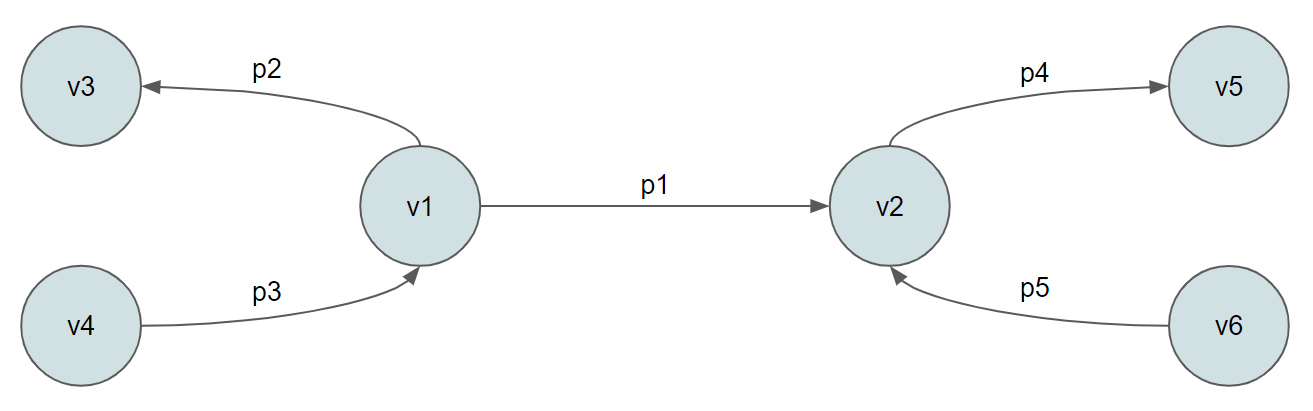
\includegraphics[width=\linewidth]{imagenes/graph2.png}
        \caption{Domain and range types graph.}
        \label{fig:example_graph2}
\end{figure}

\textbf{Aidan: I have a huge mess with formats in the doc. I have to sit down and fix it with patience.}

We will consider that any random number of elements (nodes or edges) are constant. For each of these constants, we will propagate their types: Nodes will contribute with their types to adjacent variable edges; Edges will contribute with their domain- and range-types to variable nodes.

Our first step will be to expand known types among neighbours. The following code depicts how this task is done:

\begin{minted}[linenos,tabsize=2,frame=single,samepage]{csharp}
ExpandTypes(graph){
  //We first expand node types:
  foreach (node in graph.Nodes){
    if(node.IsConstant)
      node.Types = node.URIs;
      node.ParentTypes = DB.GetParentTypes(node.URIs);
    //Get type from target instanceOf Edges:
    if(node.IsInstanceOf) 
      node.ParentTypes = node.OutInstanceOfEdges.TargetNode.Types;
  }

  //Then edge types:
  foreach(edge in graph.Edges){
    source = edge.SourceNode;
    target = edge.TargetNode;

    //Source domain types first:
    if(source.IsConstant || source.IsInstanceOf)
      edge.DomainTypes = source.ParentTypes;
    else if(edge.IsConstant)
      edge.DomainTypes = edge.GetPropertyDomainsFromDB();

    //Then target range types:
    if(target.IsConstant && edge.IsInstanceOf)
      edge.RangeTypes = target.Types;
    else if(target.IsConstant || target.IsInstanceOf)
      edge.RangeTypes = target.ParentTypes;
    else if(edge.IsConstant)
      edge.RangeTypes = edge.GetPropertyRangesFromDB();
  }
}
\end{minted}

Once we have all known types in place, we can now get values for both nodes and edges.

For nodes, we will focus on the outgoing and incoming edges. From these edges, we collect: for the outgoing edges, the domain types (our node must be inside this domain); and for the incoming edges, we collect the range types (our node must also be in this range). In other words, we are going to intersect the outgoing-edges-domain-types and the incoming-edges-range-types. A high-level detail of this process can be appreciated on the next code block:

\begin{minted}[linenos,tabsize=2,frame=single,samepage]{csharp}
GetNodesResults(graph){
  foreach (node in graph.Nodes){
    if(node.IsInstanceOf)
      node.Results = DB.GetInstancesOf(node.ParentTypes);
    else{
      domainTypes = node.OutgoingEdges.DomainTypes;
      rangeTypes = node.IncomingEdges.RangeTypes;
      node.Results = domainTypes.Intersect(rangeTypes);
    }
  }
}
\end{minted}

For edges, we will focus on both the source- and target-node of our edge. We will first do some checks on if these nodes are constants or instances of another type. If either our source or target nodes are constant, then we have certainty of the possible values that our edge can have (We have added these values directly into our DB).

If the source or target node are an instance of another type (thus a variable), then we query the outgoing or incoming properties for that type: While indexing, we have collected these properties for all instances of that type. But in this case, we also explore other possible relations existing in our graph.

Focusing in our source node, we will check all outgoing constant edges. Being constant, these edges can provide information about the values for their domains, and with these, the type of our node. We will do the same for the incoming constant edges of our source node. If there are constant incoming edges, then our node type must be in the range of those types.

We will repeat the same for the target node and then we will intersect all these known types. With this information, we are able to approximate that our edge has a known domain and a known range. During all this process, we query our local specialized index for the known types.

We also include is a high-level representation of our code for getting edge values.

\begin{minted}[linenos,tabsize=2,frame=single,samepage]{csharp}
GetEdgesResults(graph){
  foreach(edge in graph.Edges){
    source = edge.SourceNode;
    target = edge.TargetNode;

    if (source.IsConstant || target.IsConstant) {
      sourceProps = DB.GetOutgoingProperties(source.Types);
      targetProps = DB.GetIncomingProperties(target.Types);
      suggestions = sourceProps.Intersect(targetProps);
    }
    else {
      if (source.IsInstanceOf || target.IsInstanceOf) {
        sourceProps = DB.GetOutgoingProperties(source.ParentTypes);
        targetProps = DB.GetIncomingProperties(target.ParentTypes);
        suggestions = sourceProps.Intersect(targetProps);
      }

      for(sourceOutEdge in source.OutgoingEdges(IsConstant)) {
        suggestions.Intersect(DB.GetDomainProperties(sourceOutEdge.Type));
      }
      for(sourceInEdge in source.IncomingEdges(IsConstant)) {
        suggestions.Intersect(DB.GetRangeProperties(sourceInEdge.Type));
      }
      for(targetOutEdge in target.OutgoingEdges(IsConstant)) {
        suggestions.Intersect(DB.GetDomainProperties(targetOutEdge.Type));
      }
      for(targetInEdge in target.IncomingEdges(IsConstant)) {
        suggestions.Intersect(DB.GetRangeProperties(targetInEdge.Type));
      }
    }
  }
}
\end{minted}

\end{example}

After getting approximate results for both our nodes and edges, a list of entities and properties are now available. 

Something else that must be mentioned is that for remote queries: both the label and the description are retrieved from the local index and the results are returned to the user. 

\section{Application Interface}
\label{chap:api}

The last module of our system is the application interface. It will allow our system to take requests from front-end clients and use our backend.

As was mentioned before, our system supports several types of requests:
\begin{itemize}
    \item Keyword search for entities.
    \item Keyword search for properties.
    \item Keyword search for types.
    \item Get information about a Q-code entity: label, description, etc.
    \item Get information about a P-code property: label, description, etc.
    \item Query term with a SPARQL query text.
    \item Query term with a graphical representation of a SPARQL query.
\end{itemize}

The keyword search directly reverts to the specialized index. The query term works as was previously described in this chapter.

With all of these components in place, our backend can accept and respond to requests from a frontend client. In the following chapter we will describe how to integrate our system with RDFExplorer as the client in order to apply our approach for a concrete use-case.

